\documentclass[11pt,a4paper]{article}

\usepackage[T1]{fontenc}
\usepackage[utf8]{inputenc}
\usepackage{lmodern}
\usepackage{microtype}
\usepackage[a4paper,margin=22mm,headheight=15pt]{geometry}
\usepackage{booktabs}
\usepackage{tabularx}
\usepackage{array}
\usepackage{enumitem}
\usepackage{graphicx}
\usepackage{float}
\usepackage{caption}
\usepackage{siunitx}
\usepackage{xcolor}
\usepackage{tikz}
\usetikzlibrary{arrows.meta,positioning,shapes.geometric,fit}
\usepackage{pgfplots}
\pgfplotsset{compat=1.18}
\usepackage[most]{tcolorbox}
\usepackage{natbib}
\usepackage{xurl}
\usepackage[colorlinks=true,linkcolor=MGTeal,citecolor=MGTeal,urlcolor=MGTeal]{hyperref}
\usepackage[nameinlink,noabbrev]{cleveref}
\usepackage{fancyhdr}
\usepackage{lastpage}

\definecolor{MGInk}{HTML}{28251D}
\definecolor{MGMuted}{HTML}{6F6D67}
\definecolor{MGTeal}{HTML}{01696F}
\definecolor{MGTealDark}{HTML}{0C4E54}
\definecolor{MGTealLight}{HTML}{DDEDEF}
\definecolor{MGRust}{HTML}{964219}
\definecolor{MGRustLight}{HTML}{F5E7DF}
\definecolor{MGGreen}{HTML}{437A22}
\definecolor{MGGreenLight}{HTML}{E7EFE2}
\definecolor{MGRed}{HTML}{A12C7B}
\definecolor{MGRedLight}{HTML}{F7E8F1}
\definecolor{MGGrey}{HTML}{D4D1CA}
\definecolor{MGSurface}{HTML}{F7F6F2}

\color{MGInk}
\setlength{\parindent}{0pt}
\setlength{\parskip}{0.55em}
\setlength{\emergencystretch}{2em}
\setlist[itemize]{leftmargin=1.5em,itemsep=0.25em,topsep=0.25em}
\setlist[enumerate]{leftmargin=1.7em,itemsep=0.25em,topsep=0.25em}
\renewcommand{\arraystretch}{1.16}
\captionsetup{font=small,labelfont=bf}

\pagestyle{fancy}
\fancyhf{}
\lhead{\textcolor{MGMuted}{MetaboGuard progress report}}
\rhead{\textcolor{MGMuted}{11 August 2026}}
\cfoot{\textcolor{MGMuted}{\thepage\ of \pageref{LastPage}}}
\renewcommand{\headrulewidth}{0.4pt}

\newtcolorbox{summarybox}{
  colback=MGTealLight,
  colframe=MGTeal,
  boxrule=0.7pt,
  arc=2mm,
  left=3mm,right=3mm,top=2mm,bottom=2mm
}
\newtcolorbox{warningbox}{
  colback=MGRustLight,
  colframe=MGRust,
  boxrule=0.7pt,
  arc=2mm,
  left=3mm,right=3mm,top=2mm,bottom=2mm
}
\newtcolorbox{decisionbox}{
  colback=MGGreenLight,
  colframe=MGGreen,
  boxrule=0.7pt,
  arc=2mm,
  left=3mm,right=3mm,top=2mm,bottom=2mm
}

\newcommand{\status}[2]{\textcolor{#1}{\textbf{#2}}}
\newcommand{\code}[1]{\texttt{\small #1}}

\hypersetup{
  pdftitle={MetaboGuard Progress Report},
  pdfauthor={Jay Bell, KERI Department},
  pdfsubject={Self-supervised metabolic phenotyping, future-risk simulation, and clustering remediation}
}

\title{\vspace{-1.2cm}
  {\color{MGTealDark}\rule{\textwidth}{1.3pt}}\\[0.6cm]
  {\LARGE\bfseries MetaboGuard Progress Report}\\[0.25cm]
  {\large Self-supervised metabolic phenotyping, longitudinal simulation,\\
  and resolution of the biomarker clustering abstention}\\[0.6cm]
  {\color{MGTealDark}\rule{\textwidth}{0.5pt}}
}
\author{Jay Bell\\KERI Department}
\date{11 August 2026}

\begin{document}
\maketitle
\thispagestyle{empty}

\begin{summarybox}
\textbf{Executive conclusion.}
Since the 4 August meeting, MetaboGuard has moved from a cross-sectional proof of
concept to a reproducible research platform with fail-closed data checks,
label-free representation learning, evidence-linked biomarker interpretation,
exploratory clustering, a simulation-only longitudinal risk pipeline, and a
password-protected professor dashboard. The principal negative result is
scientifically useful: no candidate clustering passed all quality, stability,
outlier and nuisance-control gates. The dominant recovered structure was survey
cycle, missingness and assay availability rather than a defensible metabolic
phenotype. The correct next step is not to relax the gates. It is to harmonise
assays across cycles, test clustering within cycles against correlation-preserving
null data, transport frozen clusters to held-out cycles, and adopt continuous
latent factors if discrete clusters remain unsupported.
\end{summarybox}

\begin{warningbox}
\textbf{Clinical boundary.}
MetaboGuard remains non-diagnostic. NHANES is cross-sectional, TCGA is
post-diagnosis, and the longitudinal future-risk pipeline is trained only on
synthetic Synthea records. No output currently estimates a real patient's risk of
developing cancer or diabetes.
\end{warningbox}

\tableofcontents
\newpage

\section{Project objective and evaluation posture}

MetaboGuard investigates whether combinations of routine metabolic, biochemical
and behavioural measurements contain reproducible patterns that could support
clinician-reviewed early-warning research. The project deliberately separates
four questions:

\begin{enumerate}
  \item whether the input data are reliable and comparable;
  \item whether a label-free model learns a useful metabolic representation;
  \item whether discrete, reproducible phenotypes exist;
  \item whether a future longitudinal cohort can support calibrated event risk.
\end{enumerate}

The present report covers work completed since the 4 August 2026 professor
meeting. It uses committed repository records, frozen JSON reports and project
documentation. The current clustering report is tied to dataset fingerprint
\code{af790f9f\ldots d6b8b7c}; the deployed snapshot clusters a 16-dimensional
frozen latent representation using persisted patient-grouped splits.

\section{Changes completed since the last meeting}

\subsection{Delivery timeline}

\begin{table}[H]
\centering
\small
\caption{Major committed milestones after the 4 August meeting.}
\begin{tabularx}{\textwidth}{>{\bfseries}p{18mm} X}
\toprule
Date & Change delivered \\
\midrule
4 Aug & Fail-closed cancer coding and leakage tests; self-supervised training
tests; benchmark guide; model card; reproducibility guide. \\
4 Aug & Exploratory clustering, reliability reporting, evidence claims contract,
and documented professor feedback. \\
4--5 Aug & Synthetic patient generation, protected professor dashboard, serverless
NumPy inference, deployment security tests, Vercel configuration and Git deployment assets. \\
5 Aug & Versioned longitudinal schema, Synthea generation pipeline, future-risk
protocol, deterministic synthetic histories and simulation-only dashboard panel. \\
8 Aug & Portable future-risk export; enhanced probe interpretation; refactoring;
offline PyTorch retraining with NumPy serving compatibility. \\
\bottomrule
\end{tabularx}
\end{table}

\subsection{System architecture}

\begin{figure}[H]
\centering
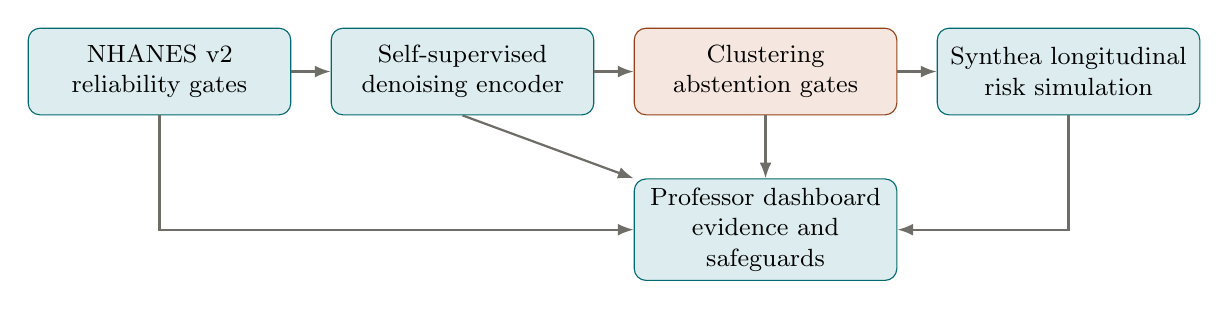
\begin{tikzpicture}[
  node distance=5mm and 5mm,
  box/.style={draw=MGGrey, rounded corners=1.5mm, fill=MGSurface,
    minimum height=11mm, text width=31mm, align=center, font=\small},
  done/.style={box, draw=MGTeal, fill=MGTealLight},
  guard/.style={box, draw=MGRust, fill=MGRustLight},
  arrow/.style={-{Latex[length=2mm]}, thick, draw=MGMuted}
]
\node[done] (data) {NHANES v2\\reliability gates};
\node[done, right=of data] (ssl) {Self-supervised\\denoising encoder};
\node[guard, right=of ssl] (cluster) {Clustering\\abstention gates};
\node[done, right=of cluster] (risk) {Synthea longitudinal\\risk simulation};
\node[done, below=8mm of cluster] (dash) {Professor dashboard\\evidence and safeguards};

\draw[arrow] (data) -- (ssl);
\draw[arrow] (ssl) -- (cluster);
\draw[arrow] (cluster) -- (risk);
\draw[arrow] (data.south) |- (dash.west);
\draw[arrow] (ssl.south) -- (dash.north west);
\draw[arrow] (cluster.south) -- (dash.north);
\draw[arrow] (risk.south) |- (dash.east);
\end{tikzpicture}
\caption{Current research architecture. Orange denotes a deliberate abstention
boundary rather than a failed software path.}
\label{fig:architecture}
\end{figure}

\subsection{Data integrity and reliability}

The reliability pipeline now records provenance, schema, plausible ranges,
duplicate handling, feature coverage, missingness by split and cycle,
assay-cycle drift, label confidence, leakage, survey-weight applicability and
capability state. The current report passes hard validation and places features
into four explicit eligibility tiers.

\begin{figure}[H]
\centering
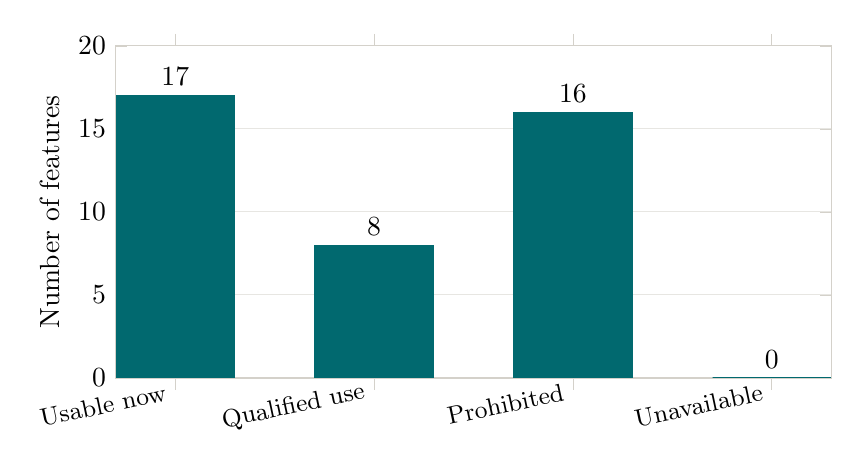
\begin{tikzpicture}
\begin{axis}[
  ybar,
  width=0.88\textwidth,
  height=58mm,
  ymin=0,ymax=20,
  ylabel={Number of features},
  symbolic x coords={Usable now,Qualified use,Prohibited,Unavailable},
  xtick=data,
  x tick label style={font=\small,rotate=12,anchor=east},
  nodes near coords,
  nodes near coords align={vertical},
  bar width=15mm,
  axis line style={draw=MGGrey},
  tick style={draw=MGGrey},
  ymajorgrids=true,
  grid style={draw=MGGrey!55},
]
\addplot[fill=MGTeal,draw=MGTeal] coordinates {
  (Usable now,17) (Qualified use,8) (Prohibited,16) (Unavailable,0)
};
\end{axis}
\end{tikzpicture}
\caption{Feature eligibility after reliability checks. Prohibited variables are
outcomes, label-derived variables or post-diagnosis context and are blocked from
the encoder.}
\label{fig:reliability}
\end{figure}

\subsection{Self-supervised representation and benchmarking}

The core model remains a label-free denoising encoder. Preprocessing is fitted
on the training partition only; split IDs, seeds, fingerprints and model metadata
are persisted. The deployment uses NumPy-exported weights, while training uses
PyTorch. PCA and Isolation Forest were added as transparent baselines. This
separation demonstrates that dependency-light serving is not equivalent to
training a NumPy-only model.

The professor dashboard adds protected access, synthetic-patient probing,
de-identified CSV validation, reliability and cluster reports, source-linked
evidence, methodology explanations and simulation-only future-risk views. No
uploaded file is retained.

\subsection{Biomarker evidence and claims contract}

A machine-readable evidence catalogue and claims contract now distinguish:

\begin{itemize}
  \item patient observations;
  \item model associations;
  \item published biomarker evidence;
  \item causal claims, which remain unestablished unless supported by an
  appropriate causal design.
\end{itemize}

This prevents diagnostic case-control biomarker performance from being
misrepresented as pre-diagnostic performance. It also prevents deviation scores,
cluster assignments and synthetic future-risk values from being described as
clinical probabilities.

\subsection{Longitudinal schema and future-risk simulation}

The new longitudinal schema represents timestamped observations, visits, index
dates, outcomes, censoring, provenance and missingness. The synthetic cohort uses
official Synthea records, which are suitable for software verification but not
clinical validation \citep{walonoski2018,chen2019synthea}.

The committed pooled cohort contains 1,542,237 event rows and 5,784 eligible
patients, with a median of 10 visits per patient. It supports only horizons that
clear the pre-specified 50-event and 50-non-event gate.

\begin{figure}[H]
\centering
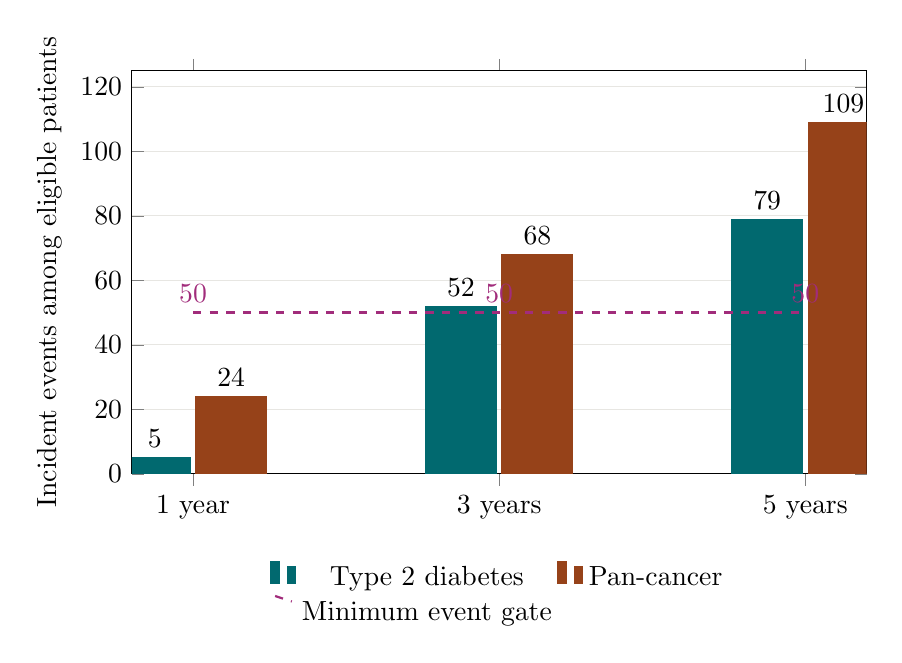
\begin{tikzpicture}
\begin{axis}[
  ybar,
  width=0.9\textwidth,
  height=67mm,
  ymin=0,ymax=125,
  ylabel={Incident events among eligible patients},
  symbolic x coords={1 year,3 years,5 years},
  xtick=data,
  legend style={at={(0.5,-0.20)},anchor=north,legend columns=2,draw=none},
  nodes near coords,
  bar width=9mm,
  ymajorgrids=true,
  grid style={draw=MGGrey!55},
]
\addplot[fill=MGTeal,draw=MGTeal] coordinates {
  (1 year,5) (3 years,52) (5 years,79)
};
\addplot[fill=MGRust,draw=MGRust] coordinates {
  (1 year,24) (3 years,68) (5 years,109)
};
\addplot[MGRed,thick,dashed,sharp plot] coordinates {
  (1 year,50) (3 years,50) (5 years,50)
};
\legend{Type 2 diabetes,Pan-cancer,Minimum event gate}
\end{axis}
\end{tikzpicture}
\caption{Synthea event counts. One-year horizons abstain; eligible horizons are
simulation-only and all held-out event counts remain small.}
\label{fig:risk-events}
\end{figure}

The risk pipeline includes horizon logistic regression, cause-specific
discrete-time hazards, gradient-boosted trees and an experimental temporal GRU.
Temporal models must lose at least 0.02 AUROC when visit order is reversed.
Type 2 diabetes GRUs failed this gate; pan-cancer GRUs passed at three and five
years. Every metric is explicitly marked synthetic and underpowered, and the
clinical endpoint remains HTTP 409.

\section{Primary finding: no defensible biomarker clusters}

\subsection{What the current run found}

The deployed clustering report uses 4,000 training rows, five bootstrap rounds
and K-means with \(K=2,3,4\). All candidates fail at least one gate.

\begin{table}[H]
\centering
\small
\caption{Exact clustering diagnostics from the committed all-adults report.}
\begin{tabular}{lrrrrp{46mm}}
\toprule
Candidate & Silhouette & Bootstrap ARI & Min.\ Jaccard & Cycle \(V\) & Main failures \\
\midrule
K-means \(K=2\) & 0.492 & 0.238 & 0.305 & 0.482 &
Cycle dominated; unstable; one cluster dissolves. \\
K-means \(K=3\) & 0.389 & 0.450 & 0.414 & 0.281 &
Tiny cluster; missingness dominated; outlier sensitive. \\
K-means \(K=4\) & 0.253 & 0.965 & 0.867 & 0.495 &
Tiny cluster; cycle, missingness and assay dominated; outlier sensitive. \\
\bottomrule
\end{tabular}
\label{tab:cluster-results}
\end{table}

The result is \code{no\_stable\_clusters}. This is not a contradiction:
\(K=4\) has strong geometric stability but fails validity controls, while \(K=2\)
has adequate geometric separation but fails resampling stability and cycle
control. Stable clusters can still be stable artefacts \citep{hennig2007};
consensus procedures can find crisp partitions in correlation-preserving null
data \citep{senbabaoglu2014,m3c2020}.

\subsection{Why this happened}

\begin{figure}[H]
\centering
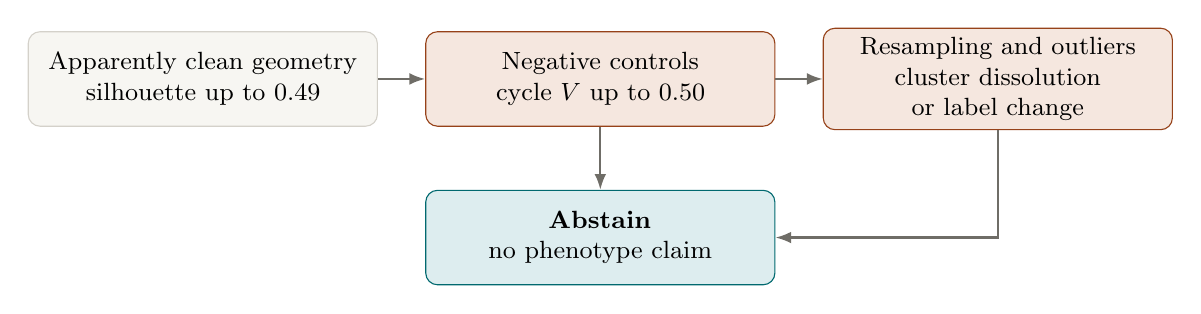
\begin{tikzpicture}[
  node distance=6mm,
  stagebox/.style={draw=MGGrey, rounded corners=1.5mm, fill=MGSurface,
    text width=42mm, minimum height=12mm, align=center, font=\small},
  fail/.style={stagebox, draw=MGRust, fill=MGRustLight},
  result/.style={stagebox, draw=MGTeal, fill=MGTealLight},
  arrow/.style={-{Latex[length=2mm]}, thick, draw=MGMuted}
]
\node[stagebox] (clean) {Apparently clean geometry\\silhouette up to 0.49};
\node[fail, right=of clean] (nuis) {Negative controls\\cycle \(V\) up to 0.50};
\node[fail, right=of nuis] (stab) {Resampling and outliers\\cluster dissolution or label change};
\node[result, below=8mm of nuis] (abstain) {\textbf{Abstain}\\no phenotype claim};
\draw[arrow] (clean) -- (nuis);
\draw[arrow] (nuis) -- (stab);
\draw[arrow] (nuis) -- (abstain);
\draw[arrow] (stab) |- (abstain);
\end{tikzpicture}
\caption{Why the abstention is a safety success. Geometry is evaluated before,
but never allowed to override, nuisance and stability checks.}
\label{fig:abstention}
\end{figure}

The most likely causes are:

\begin{enumerate}
  \item \textbf{Assay and protocol changes across cycles.} NHANES documents
  instrument changes and publishes bridging equations for some biomarkers,
  including insulin \citep{nhanesInsulin}.
  \item \textbf{Structural missingness and subsampling.} Fasting analytes and
  specialist assays are available only in subsamples and selected cycles.
  \item \textbf{Pooling before harmonisation.} Cycle is a large, structured signal;
  official guidance requires method comparability and appropriate multi-cycle
  weights before combining data \citep{nhanesWeights,nhanesQuality}.
  \item \textbf{Possibly continuous rather than discrete biology.} A metabolic
  gradient may be real even when hard clusters are not. Continuous clinical
  variables can outperform patient subgroup labels for prognosis and treatment
  selection \citep{dennis2019}.
  \item \textbf{Biomarker coverage.} Routine NHANES measurements do not include a
  consistent multi-omics panel or verified pre-diagnostic cancer outcomes.
\end{enumerate}

\begin{decisionbox}
\textbf{Interpretation for the paper.}
The current result should be reported as: ``No discrete metabolic phenotype
passed the pre-specified validity gates in pooled, unharmonised multi-cycle
NHANES.'' It should not be reported as: ``metabolic phenotypes do not exist.''
\end{decisionbox}

\section{Plan to resolve the clustering issue}

\subsection{P0: establish whether the signal survives harmonisation}

\begin{enumerate}
  \item \textbf{Freeze an analyte-by-cycle provenance table.} Record instrument,
  method, limit of detection, age eligibility, fasting requirement, subsample
  weight and bridging equation for every feature. Use only features with stable
  methods or documented conversion equations \citep{nhanesQuality}.
  \item \textbf{Create raw and harmonised matrices.} Apply CDC bridging equations
  first, then transformation and scaling. Compare pooled robust scaling with
  within-cycle robust scaling.
  \item \textbf{Require nuisance reduction before clustering.} A cross-validated
  survey-cycle classifier should have AUC \(\leq 0.60\). Cycle association for a
  promoted cluster should be \(V \leq 0.20\).
  \item \textbf{Split cycles into discovery and held-out sets.} No held-out cycle
  may influence preprocessing, K selection or hyperparameters.
\end{enumerate}

\subsection{P0: test cluster existence against a matched null}

Run K-means, Gaussian mixtures and fuzzy c-means within each discovery cycle for
\(K=2,\ldots,8\), with at least 25 seeds. Classical consensus clustering is not
enough because it can partition cluster-less data \citep{senbabaoglu2014}. Use
M3C-style correlation-preserving null datasets and at least 100 Monte Carlo
replicates \citep{m3c2020}.

Promote a discrete phenotype only when:

\begin{itemize}
  \item Monte Carlo \(p<0.05\) at \(K\), with adjacent \(K-1\) and \(K+1\)
  nulls also rejected;
  \item every cluster is at least 5\% and contains at least 30 participants in
  every included cycle;
  \item bootstrap ARI, seed ARI and outlier/noise-replacement ARI are each
  at least 0.60;
  \item cluster-wise mean Jaccard is at least 0.75, raising the present threshold
  from ``not dissolved'' to ``well recovered'' \citep{hennig2007};
  \item cross-cycle transport ARI is at least 0.60;
  \item nuisance associations remain below pre-specified thresholds and their
  null distributions.
\end{itemize}

\subsection{P0/P1: treat missingness and survey design explicitly}

Use three parallel missing-data analyses:

\begin{enumerate}
  \item complete-case clustering within common assay-availability strata;
  \item multiple imputation with at least 20 completed datasets and a documented
  MAR/MNAR sensitivity analysis \citep{sterne2009,vanbuuren2011};
  \item a latent-variable model with native missing-modality handling.
\end{enumerate}

Cluster discovery can remain unweighted as a declared exploratory analysis, but
cluster prevalences and associations must use the NHANES weight, PSU and strata
design. NCHS shows that unweighted estimates can differ materially from
design-weighted estimates \citep{nhanesWeights,nhanesVariance}.

\subsection{P1/P2: external and longitudinal validation}

Freeze the selected centroids or posterior model and assign held-out cycles
without refitting. A transported cluster must add predictive information beyond
a continuous-feature comparator. This matters because externally replicated
diabetes clusters have not consistently outperformed simple continuous
predictors \citep{ahlqvist2018,dennis2019}.

If compatible clinical, metabolomic, proteomic and genetic blocks become
available, use multi-view factor analysis first and similarity network fusion
only on a defensible shared subsample \citep{mofa2018,snf2014}. A real
longitudinal cohort remains necessary to test incident outcomes.

\subsection{Pre-registered continuous fallback}

If the null of one continuous population cannot be rejected after P0
harmonisation, the project should not force clusters. The fallback deliverable is
a continuous metabolic factor or graded membership score. This is still aligned
with early-warning research and may be more useful than hard subgroup labels
\citep{dalmaijer2022,dennis2019}.

\section{Eight-week delivery plan}

\begin{table}[H]
\centering
\small
\caption{Recommended work programme to resolve the clustering question.}
\begin{tabularx}{\textwidth}{>{\bfseries}p{13mm} p{37mm} X p{31mm}}
\toprule
Week & Workstream & Main actions & Deliverable / gate \\
\midrule
1 & Provenance and design freeze &
Analyte-cycle table; survey design; discovery/held-out cycles; seal outcomes;
register all methods and gates. &
Frozen analysis plan. \\
2 & Harmonisation &
CDC bridging equations; feature intersection; pooled and within-cycle
standardisation; nuisance classifiers. &
Cycle AUC \(\leq 0.60\). \\
3 & Null calibration &
Intercept-only ComBat sensitivity; 100 correlation-preserving null datasets;
null distributions for silhouette, PAC, DB, CH and ARI. &
Null reference table. \\
4 & Missingness arms &
Availability-stratified complete cases; 20+ imputations; native-missing factor
model; compare assignments. &
Across-imputation ARI and missingness verdict. \\
5 & Within-cycle discovery &
\(K=2\ldots8\), multiple algorithms, 25+ seeds, M3C tests, 50+ stability
resamples and noise replacement. &
First formal go/no-go. \\
6 & Cross-cycle consensus &
Transport centroids/posteriors between discovery cycles; continuous multi-view
factors as fallback. &
Cross-cycle ARI matrix. \\
7 & Held-out transport &
Assign untouched cycles without refitting; design-weighted cluster prevalence
and uncertainty. &
Transport report. \\
8 & Outcome validation &
Unseal outcomes once; compare clusters against continuous features; final
decision and paper-ready negative result if needed. &
Decision memo and manuscript update. \\
\bottomrule
\end{tabularx}
\end{table}

\section{Risks, decisions and requests to the team}

\begin{table}[H]
\centering
\small
\begin{tabularx}{\textwidth}{>{\bfseries}p{34mm} X}
\toprule
Decision requested & Recommendation \\
\midrule
Primary clustering objective &
Approve a formal cluster-existence test, not a target number of clusters. \\
Cycle window &
Select cycles with the strongest assay comparability; hold later cycles out. \\
Survey statistics support &
Assign biostatistical review for multi-cycle weights, PSU/strata inference and
multiple imputation. \\
Cluster gate update &
Raise promoted-cluster Jaccard to 0.75 and replace a fixed null-gain rule with a
Monte Carlo \(p\)-value. \\
Fallback product &
Pre-approve a continuous metabolic factor if discrete clusters remain unsupported. \\
External data &
Prioritise access to a real longitudinal cohort and consistent multi-omics blocks. \\
\bottomrule
\end{tabularx}
\end{table}

\section{Conclusion}

The project has made substantial engineering and methodological progress:
corrected data, leakage controls, reproducible self-supervised training,
transparent baselines, evidence provenance, cautious clustering, a versioned
longitudinal simulation pipeline and a professor-facing deployment. The
clustering abstention is the most important finding because it prevents a
plausible-looking but invalid phenotype claim.

The next phase should answer a narrower and publishable question:
\emph{after assay harmonisation, complex-survey handling and
correlation-preserving null calibration, is there evidence for discrete,
transportable metabolic phenotypes?} If the answer remains no, a continuous
factor model is the scientifically correct output.

\appendix

\section{Metric glossary}

\begin{tabularx}{\textwidth}{>{\bfseries}p{34mm} X}
\toprule
Metric & Interpretation \\
\midrule
Silhouette & Separation relative to within-cluster compactness. Must be compared
with a matched null; high values alone do not establish biological structure. \\
Adjusted Rand index & Chance-corrected agreement between two assignments. Used
for seeds, bootstrap refits, outlier sensitivity and cross-cycle transport. \\
Cluster-wise Jaccard & Recovery of each individual cluster after resampling.
Values \(\leq0.50\) indicate dissolution; \(\geq0.75\) is the proposed promotion gate. \\
Cramér's \(V\) & Association between cluster labels and categorical nuisance
variables such as survey cycle. \\
Permutation/null gain & Difference between the observed cluster metric and a
correlation-preserving null distribution. \\
\bottomrule
\end{tabularx}

\section{Safe statements for presentations and/or showcases}

\begin{itemize}
  \item ``The system found candidate geometric partitions, but none passed all
  stability and nuisance-control gates.''
  \item ``The dominant recoverable structure was survey-cycle and assay
  availability, not a validated biological phenotype.''
  \item ``The abstention is a safety result, not a software failure.''
  \item ``Future-risk functionality has been engineered and tested on synthetic
  longitudinal records only; it is not a patient-risk model.''
  \item ``The next experiment will test cluster existence after harmonisation
  against a correlation-preserving null and held-out cycles.''
\end{itemize}

\begin{thebibliography}{99}

\bibitem[Ahlqvist et~al.(2018)]{ahlqvist2018}
E. Ahlqvist et al.
\newblock Novel subgroups of adult-onset diabetes and their association with outcomes.
\newblock \emph{Lancet Diabetes \& Endocrinology}, 2018.
\newblock \href{https://doi.org/10.1016/S2213-8587(18)30051-2}{doi:10.1016/S2213-8587(18)30051-2}.

\bibitem[Chen et~al.(2019)]{chen2019synthea}
J. Chen et al.
\newblock Validation of a synthetic data set.
\newblock \emph{BMC Medical Informatics and Decision Making}, 2019.
\newblock \href{https://doi.org/10.1186/s12911-019-0793-0}{doi:10.1186/s12911-019-0793-0}.

\bibitem[Dalmaijer et~al.(2022)]{dalmaijer2022}
E. S. Dalmaijer, C. L. Nord, and D. E. Astle.
\newblock Statistical power for cluster analysis.
\newblock \emph{BMC Bioinformatics}, 23:205, 2022.
\newblock \href{https://doi.org/10.1186/s12859-022-04675-1}{doi:10.1186/s12859-022-04675-1}.

\bibitem[Dennis et~al.(2019)]{dennis2019}
J. M. Dennis et al.
\newblock Disease progression and treatment response in data-driven subgroups of type 2 diabetes.
\newblock \emph{Lancet Diabetes \& Endocrinology}, 2019.
\newblock \href{https://doi.org/10.1016/S2213-8587(19)30087-7}{doi:10.1016/S2213-8587(19)30087-7}.

\bibitem[Hennig(2007)]{hennig2007}
C. Hennig.
\newblock Cluster-wise assessment of cluster stability.
\newblock \emph{Computational Statistics \& Data Analysis}, 52(1):258--271, 2007.
\newblock \url{https://www.homepages.ucl.ac.uk/~ucakche/papers/clusta.pdf}.

\bibitem[Johnson et~al.(2007)]{combat2007}
W. E. Johnson, C. Li, and A. Rabinovic.
\newblock Adjusting batch effects in microarray expression data using empirical Bayes methods.
\newblock \emph{Biostatistics}, 8(1):118--127, 2007.
\newblock \href{https://doi.org/10.1093/biostatistics/kxj037}{doi:10.1093/biostatistics/kxj037}.

\bibitem[Monti et~al.(2003)]{monti2003}
S. Monti, P. Tamayo, J. Mesirov, and T. Golub.
\newblock Consensus clustering: a resampling-based method for class discovery.
\newblock \emph{Machine Learning}, 52:91--118, 2003.
\newblock \href{https://doi.org/10.1023/A:1023949509487}{doi:10.1023/A:1023949509487}.

\bibitem[Senbabaoglu et~al.(2014)]{senbabaoglu2014}
Y. Senbabaoglu, G. Michailidis, and J. Z. Li.
\newblock Critical limitations of consensus clustering in class discovery.
\newblock \emph{Scientific Reports}, 4:6207, 2014.
\newblock \href{https://doi.org/10.1038/srep06207}{doi:10.1038/srep06207}.

\bibitem[John et~al.(2020)]{m3c2020}
C. R. John et al.
\newblock M3C: Monte Carlo reference-based consensus clustering.
\newblock \emph{Scientific Reports}, 2020.
\newblock \url{https://www.nature.com/articles/s41598-020-58766-1}.

\bibitem[Sterne et~al.(2009)]{sterne2009}
J. A. C. Sterne et al.
\newblock Multiple imputation for missing data in epidemiological and clinical research.
\newblock \emph{BMJ}, 338:b2393, 2009.
\newblock \href{https://doi.org/10.1136/bmj.b2393}{doi:10.1136/bmj.b2393}.

\bibitem[van Buuren and Groothuis-Oudshoorn(2011)]{vanbuuren2011}
S. van Buuren and K. Groothuis-Oudshoorn.
\newblock mice: Multivariate Imputation by Chained Equations in R.
\newblock \emph{Journal of Statistical Software}, 45(3), 2011.
\newblock \href{https://doi.org/10.18637/jss.v045.i03}{doi:10.18637/jss.v045.i03}.

\bibitem[Walonoski et~al.(2018)]{walonoski2018}
J. Walonoski et al.
\newblock Synthea: an approach, method, and software mechanism for generating synthetic patients.
\newblock \emph{Journal of the American Medical Informatics Association}, 2018.
\newblock \href{https://doi.org/10.1093/jamia/ocx079}{doi:10.1093/jamia/ocx079}.

\bibitem[Argelaguet et~al.(2018)]{mofa2018}
R. Argelaguet et al.
\newblock Multi-Omics Factor Analysis.
\newblock \emph{Molecular Systems Biology}, 14:e8124, 2018.
\newblock \href{https://doi.org/10.15252/msb.20178124}{doi:10.15252/msb.20178124}.

\bibitem[Wang et~al.(2014)]{snf2014}
B. Wang et al.
\newblock Similarity network fusion for aggregating data types on a genomic scale.
\newblock \emph{Nature Methods}, 11:333--337, 2014.
\newblock \href{https://doi.org/10.1038/nmeth.2810}{doi:10.1038/nmeth.2810}.

\bibitem[NCHS(2026a)]{nhanesWeights}
National Center for Health Statistics.
\newblock NHANES weighting tutorial.
\newblock \url{https://wwwn.cdc.gov/nchs/nhanes/tutorials/weighting.aspx}.

\bibitem[NCHS(2026b)]{nhanesVariance}
National Center for Health Statistics.
\newblock NHANES variance estimation tutorial.
\newblock \url{https://wwwn.cdc.gov/nchs/nhanes/tutorials/VarianceEstimation.aspx}.

\bibitem[NCHS(2026c)]{nhanesQuality}
National Center for Health Statistics.
\newblock Guidelines for high quality analyses of NHANES data.
\newblock \url{https://wwwn.cdc.gov/nchs/nhanes/QualityAnalysesGuidelines.aspx}.

\bibitem[NCHS(2011)]{nhanesInsulin}
National Center for Health Statistics.
\newblock NHANES 2011--2012 fasting glucose and insulin laboratory documentation.
\newblock \url{https://wwwn.cdc.gov/Nchs/Data/Nhanes/Public/2011/DataFiles/GLU_G.htm}.

\end{thebibliography}

\end{document}
